\documentclass[
  captions=tableheading,
  bibliography=totoc, 
  titepage=firstiscover,
]{scrartcl}

\usepackage{blindtext} %neuer input

\usepackage{longtable} % Tabellen über mehrere Seiten

\usepackage[utf8]{inputenc} %neuer input

\usepackage{scrhack}

\usepackage[aux]{rerunfilecheck} %Warnung falls nochmal kompiliert werden muss

\usepackage{fontspec} %Fonteinstellungen

\recalctypearea{}

\usepackage[main=ngerman]{babel} %deutsche Spracheinstellung

\usepackage{ragged2e} %neuer input

\usepackage{amsmath, nccmath}

\usepackage{amssymb} %viele mathe Symbole

\usepackage{mathtools} %Erweiterungen für amsmath


\DeclarePairedDelimiter{\abs}{\lvert}{\rvert}
\DeclarePairedDelimiter{\norm}{\lVert}{\rVert}

\DeclarePairedDelimiter{\bra}{\langle}{\rvert}
\DeclarePairedDelimiter{\ket}{\lvert}{\rangle}

\DeclarePairedDelimiterX{\braket}[2]{\langle}{\rangle}{
#1 \delimsize| #2
}

\NewDocumentCommand \dif {m}
{
\mathinner{\symup{d} #1}
}


\usepackage[
  math-style=ISO,
  bold-style=ISO,
  sans-style=italic,
  nabla=upright,
  partial=upright,
  warnings-off={
    mathtools-colon,
    mathtools-overbracket,
  },
]{unicode-math}

\setmathfont{Latin Modern Math}
\setmathfont{XITS Math}[range={scr, bfscr}]
\setmathfont{XITS Math}[range={cal, bfcal}, StylisticSet=1]


\usepackage[
  locale=DE,
  separate-uncertainty=true,
  per-mode=reciprocal,
  output-decimal-marker={,},
]{siunitx}

\usepackage[autostyle]{csquotes} %richtige Anführungszeichen

\usepackage{xfrac}

\usepackage{float}

\floatplacement{figure}{htbp}

\floatplacement{table}{htbp}

\usepackage[ %floats innerhalb einer section halten
  section,   %floats innerhalb er section halten
  below,     %unterhalb der Section aber auf der selben Seite ist ok
]{placeins}

\usepackage[
  labelfont=bf,
  font=small,
  width=0.9\textwidth,
]{caption}

\usepackage{subcaption} %subfigure, subtable, subref

\usepackage{graphicx}

\usepackage{grffile}

\usepackage{booktabs}

\usepackage{microtype} %Verbesserungen am Schriftbild

\usepackage[
backend=biber,
]{biblatex}

\addbibresource{../lit.bib}

\usepackage[ %Hyperlinks im Dokument
  german,
  unicode,
  pdfusetitle,
  pdfcreator={},
  pdfproducer={},
]{hyperref}

\usepackage{bookmark}

\usepackage[shortcuts]{extdash}

%\usepackage{warpcol}


\begin{document}
    \title{ATP Übungsblatt 4}
    \author{  
    Tobias Rücker\\
    \texorpdfstring{\href{mailto:tobias.ruecker@tu-dortmund.de}{tobias.ruecker@tu-dortmund.de}
    \and}{,} 
    Paul Störbrock\\
    \texorpdfstring{\href{mailto:paul.stoerbrock@tu-dortmund.de}{paul.stoerbrock@tu-dortmund.de}}{}
    }
\maketitle
\center{\Large Abgabegruppe: \textbf{Mittw. 10-12 Uhr}}
\thispagestyle{empty}

\newpage
\tableofcontents
\thispagestyle{empty}
\newpage

\setcounter{page}{1}


\section{Aufgabe 10}

    \begin{figure}[H]
        \centering
        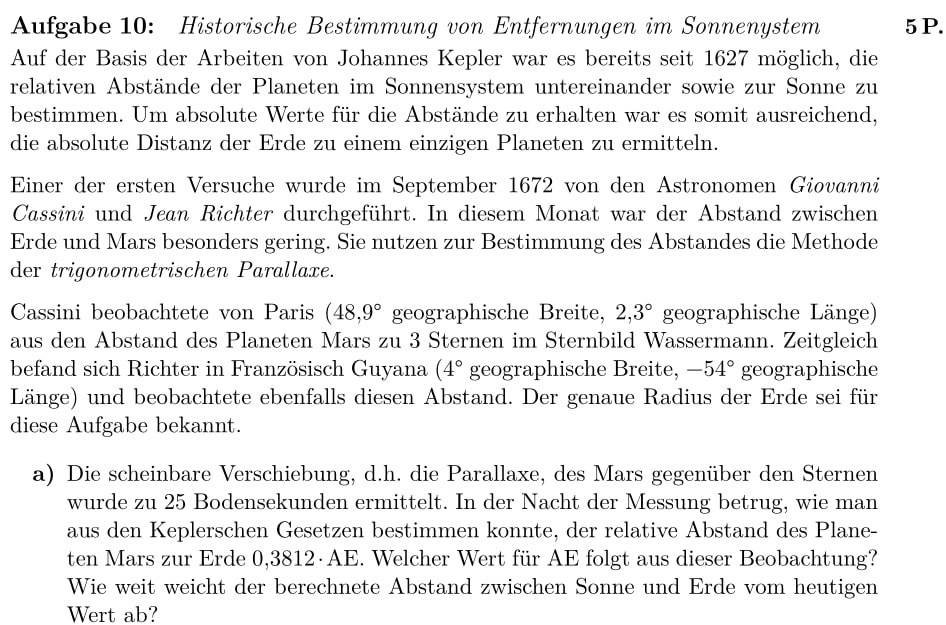
\includegraphics[width=\textwidth]{images/Aufgabe10.jpg}
        \label{fig:1}
    \end{figure}

\section{Aufgabe 11}

    \begin{figure}[H]
        \centering
        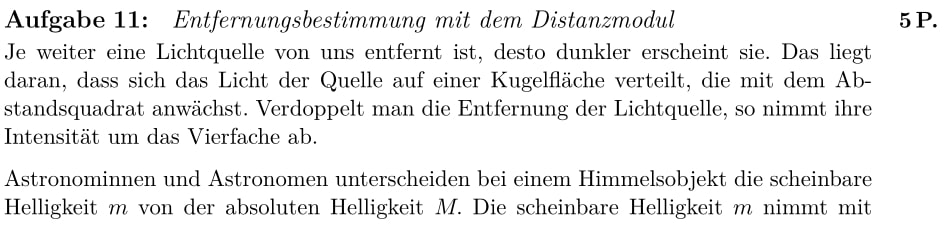
\includegraphics[width=\linewidth]{images/Aufgabe11_1.jpg}
        \label{fig:2}
    \end{figure}

    \begin{figure}[H]
        \centering
        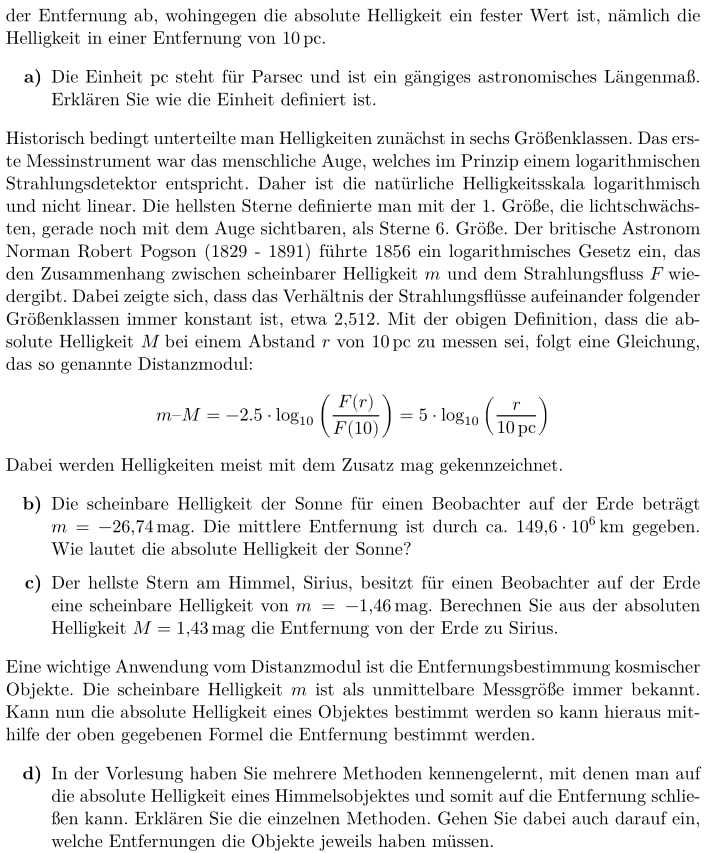
\includegraphics[width=\linewidth]{images/Aufgabe11_2.jpg}
        \label{fig:3}
    \end{figure}

    \begin{figure}[H]
        \centering
        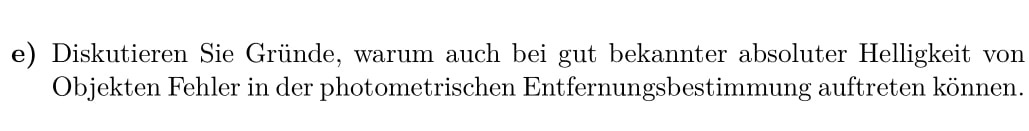
\includegraphics[width=\linewidth]{images/Aufgabe11_3.jpg}
        \label{fig:4}
    \end{figure}

    \subsection{a)}

    \subsection{b)}

    \subsection{c)}

    \subsection{d)}

    \subsection{e)}

\section{Aufgabe 12}

    \begin{figure}[H]
        \centering
        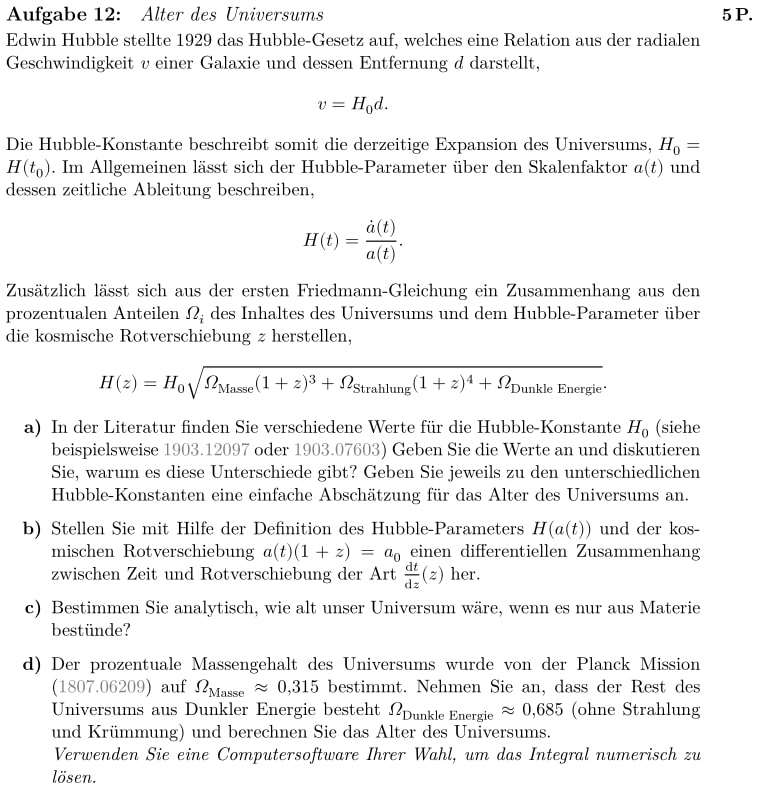
\includegraphics[width=\textwidth]{images/Aufgabe12.jpg}
        \label{fig:5}
    \end{figure}

    \subsection{a)}
    Zwei Werte aus verschiedenen Messungen für die Hubbelkonstanten sind
    \begin{align}
        H_{0,1903.12097} &= 67.4^{+6.0}_{\--6.2} \si{\kilo\meter\second\tothe{-1}\mega pc \tothe{-1}}\\
        H_{0,1903.07603} &= 74.22\pm1.82 \si{\kilo\meter\second\tothe{-1}\mega pc \tothe{-1}}
    \end{align}
    Die erste Hubbelkonstante entstammt aus einer Messung der Planck-Sonde im Jahr 2013. Diese
    hatte die Hubblekonstante und die Materiedichte des Universums über die Abschwächung hochenergetischer
    Gammaquanten. Die Menge an Gammaquanten hängt in einer Sichtlinie hängt von der Expansionsrate des
    Universums und der Materiedichte ab.\\
    Die zweite Hubblekonstante ist vom Hubble-Weltraumteleskop gemessen worden. Dabei wurden 70 langperiodige
    Cepheiden in der Magellanschen Wolke beobachtet.\\
    Diese hohe Abweichung zwischen den Messwerten ist sehr ungewöhnlich. Zum aktuellen Zeitpunkt gibt
    es keine Erklärungen für die Ursache. Ein Fehler in den Messungen ist dabei schon ausgeschlossen worden.
    Daher wird angenommen, dass es sich dabei um ein kosmische Eigenschaft handelt außerhalb des LambdaCDM
    \subsection{b)}
    \begin{align}
        H(a(t)) &= \frac{\dot{a}(t)}{a(t)}\\
        a(t) &= \frac{a_0}{1+z}\\
        \dot{a} &= \frac{\dif{}}{\dif{t}} \frac{a_0}{1+z}\\
        &= a_0 \frac{\dif{z} }{\dif{t}} \left(-\frac{1}{(1+z)^2} \right)\\
        H(z) &= \frac{-\frac{a_0}{(1+z)^2 \frac{\dif{z}}{\dif{t}}}}{\frac{a_0}{1+z}}\\
        H(z) dt &= -\frac{1}{1+z} \dif{z}\\
        \frac{dif{t}}{\dif{z}}(z)&= -\frac{1}{H(z)(1+z)}
    \end{align}

    \subsection{c)}
    Betrachtung, dass unser Universum nur aus Materie bestehe:
    \begin{align}
        \Omega _{\text{Dunkle Energie}} &= \Omega _{\text{Strahlung}} =0\\
        \Omega _{\text{Materie}} &=1\\
        H(z) &= H_0 \sqrt{(1+z)^3}\\
        \frac{\dif{t}}{\dif{z}}&=-\frac{1}{H_0 \sqrt{(1+z)^5}} 
        \dif{t} &= -\frac{1}{H_0 \sqrt{(1+z)^5}} \dif{z} \left| \int \right. \\
        \int_t^0 \dif{t'} &= -\frac{1}{H_0}  \int_0^{\infty} \frac{1}{(1+z)^{\frac{5}{2}}} \dif{z}\\
        \intertext{\justifying
            In der Gleichung vorher eird das Alter das Universum berechnet, indem vom aktuellen
            Stand zurückgerechnet wird. Dabei gilt für die größte Rotverschiebung z, das früheste
            Stadium des Universums betrachtet wird und bei der kleinsten der aktuelle Stand.
        }
        u=&z+1 \\
        &= -\frac{1}{H_0} \left(-\frac{2}{3} \right) \left(u \right)^{-\frac{3}{2}} \left|_{\infty}^1 \right. \\
        &=\frac{2}{3 H_0}
    \end{align}

    \subsection{d)}

\end{document}